%! Author = Omar Iskandarani
%! Date = 2/15/2025

\documentclass[aps,preprint,superscriptaddress]{revtex4}
\usepackage[none]{hyphenat}
\usepackage{array}
\usepackage{booktabs}
\usepackage{amsmath}
\usepackage{amssymb}
\usepackage{graphicx}
\usepackage{hyperref}
\usepackage{physics}

\begin{document}
\sloppy
\author{Omar Iskandarani}
\title{The Vortex Æther Model: Æther Vortex Field Model}
\date{\today}
\affiliation{Independent Researcher, Groningen, The Netherlands}
\thanks{ORCID: \href{https://orcid.org/0009-0006-1686-3961}{0009-0006-1686-3961}}
\email{info@omariskandarani.com}


%! Author = mr
%! Date = 4/2/2025


\begin{abstract}
This paper introduces a fluid-dynamic reformulation of general relativity through the Vortex \AE ther Model (VAM), a framework in which gravitation and time dilation arise not from spacetime curvature but from vorticity-induced pressure gradients in an effectively incompressible, inviscid superfluid medium. Within this three-dimensional, Euclidean, and temporally absolute æther, spacetime dynamics are encoded in conserved vortex structures: velocity fields, circulation constants, and topologically stable knots.
We derive analogs to Schwarzschild and Kerr metrics using the energetic and inertial properties of quantized vortex filaments, replacing geodesic motion with streamlines along conserved vorticity flux. Gravitational attraction emerges from Bernoulli-like pressure deficits generated by intense swirl regions, establishing a direct mechanical analog to gravitational potential.
Thermodynamic consistency is ensured by embedding Clausius entropy within vortex knot structures, providing an entropic interpretation of mass and time dilation. Notably, we reinterpret quantum effects such as the photoelectric effect and low-energy nuclear reactions (LENR) as resonant transitions within confined vortex networks.
This approach extends analogue gravity programs initiated by Barceló, Visser, and Volovik~\cite{barcelo2011analogue,volovik2009universe}, but introduces a topologically conserved vorticity formalism that unifies kinematic, thermodynamic, and gravitational phenomena. VAM offers a post-relativistic, energetically grounded, and experimentally accessible candidate for emergent gravity in structured continua.
\end{abstract}

\maketitle

\subsection*{The Æther Revisited: From Historical Substrate to Vorticity Field}
The term \textit{Æther} traditionally denoted an all-pervading medium facilitating wave propagation, from antiquity through 19th-century theories of luminiferous æther. By the late 1800s, Kelvin and Tait proposed vortex atom models, anticipating matter as stable, knotted structures in an ideal fluid. However, with the rise of Einstein’s relativity and the null results of the Michelson--Morley experiment, the æther concept fell into disuse---replaced by the curvature of spacetime.
Yet modern physics has quietly revived the idea in new guises: Dirac envisioned a quantum vacuum substrate; quantum field theory predicts a nontrivial ground state; and analogue gravity models---such as those of Volovik and Barceló---invoke superfluid or condensate-based media to model relativistic effects.
The Vortex Æther Model (VAM) reclaims the æther not as a particulate medium but as a topologically structured, inviscid superfluid. Here, the fundamental actors are vorticity fields: $\vec{\omega} = \nabla \times \vec{v}$ which encode rotational dynamics and replace both spacetime curvature and mass-energy density as mediators of force.
In VAM, particles correspond to topologically conserved vortex knots (e.g., trefoils, Hopf links), while gravity and inertia emerge from pressure gradients generated by swirling flow. This reframes mass as rotational energy, time dilation as a Bernoulli-pressure effect, and gravitational attraction as a vorticity-induced pressure well---providing a unified fluid-mechanical ontology for relativistic and quantum behavior.

\section*{Postulates of the Vortex \AE ther Framework}
The Vortex \AE ther Model posits a classical, three-dimensional continuum governed by fluid dynamics and topological conservation. These postulates form the foundational structure from which analogues to general relativity and quantum mechanics emerge in subsequent sections.

\begin{table}[h!]
    \centering
    \begin{tabular}{rl}
        \toprule
        \hline
        \textbf{Postulates} & of the Vortex \AE ther Model (VAM).\\
        \hline
        \textbf{1. Continuum Space} & Space is a Euclidean, incompressible, inviscid fluid medium. \\
        \midrule
        \textbf{2. Knotted Particles} & Matter arises from stable, topologically conserved vortex knots. \\
        \midrule
        \textbf{3. Vortex Dynamics} & Vorticity is conserved and quantized across the continuum. \\
        \midrule
        \textbf{4. Absolute Time} & Time flows uniformly throughout the æther. \\
        \midrule
        \textbf{5. Local Time} & Clock rates vary locally due to pressure and vorticity gradients. \\
        \midrule
        \textbf{6. Gravity} & Emerges from pressure gradients induced by localized vorticity. \\
        \hline
        \bottomrule
    \end{tabular}
    \caption{Postulates of the Vortex Æther Model (VAM).\\}
    These principles replace spacetime curvature with structured rotational flow, \\
    forming the foundation for VAM analogues to mass, time, inertia, and gravity.
    \label{tab:postulates}
\end{table}


\subsection*{VAM Constants and Scaling}

The Vortex Æther Model (VAM) is anchored by a small set of universal constants that replace geometric curvature with fluid-dynamic quantities. These include:

\begin{table}[htbp]
    \centering
    \begin{tabular}{llc}
        \hline
        \textbf{Symbol} & \textbf{Name} & \textbf{Approx. Value} \\
        \hline
        $C_e$ & Core tangential velocity & $1.09384563 \times 10^6$ m/s \\
        $r_c$ & Vortex core radius (Coulomb barrier) & $1.40897017 \times 10^{-15}$ m \\
        $F_{\max}$ & Maximum vortex-interaction (Coulomb force) & $29.053507$ N \\
        $\rho_{\text{\ae}}$ & Æther density (Universal) & $3.89343582 \times 10^{18}$ kg/m$^3$ \\
        $\alpha$ & Fine-structure constant $= \frac{2 C_e}{c}$ (emergent)   & $7.2973525643 \times 10^{-3}$\\
        $R_e$ & Electron radius ($2 \times r_c$) & $2.81794092 \times 10^{-15}$ m \\
        $G_{\text{swirl}}$ & Derived from Æther properties, proportional to $C_e$ & $ \propto \rho_{\text{\ae}} C_e^2$ or $ \propto \frac{C_e}{r_c^2}$  \\
        $\alpha_g$ &   Gravitational coupling constant & $1.7518e-45$ \\
        $\gamma$  & Vorticity-gravity coupling ($G \cdot \rho_{\ae}^2$) & $3.27 \times 10^{-23}$  m$^5$/s$^2$\\
        $\kappa$  & Circulation quantum  ($C_e \cdot r_c$) & $1.54 \times 10^{-9}$  m$^2$/s     \\
        $\beta$  & Time-dilation coupling  ($r_c^2 / C_e^2$) & $1.66 \times 10^{-42}$  s$^2$      \\
        \hline
    \end{tabular}
    \caption{Fundamental VAM constants defined in prior work \cite{vam2025field, vam2025unified}.}\label{tab:table}
\end{table}



\subsection*{Planck-Scale Derivation of Maximum Vortex Force}

The maximum allowable force between vortex structures in VAM is derived from Planck-scale physics, scaled by the fine-structure constant and the geometric ratio of the vortex core to the Planck length:

\[
F_{\text{max}} = \frac{c^4}{4G} \cdot \alpha \cdot \left( \frac{r_c}{L_p} \right)^{-2}
\]

Using defined constants, this yields precisely:

\[
F_{\text{max}} = 29.053507~\text{N}
\]

This links the VAM-specific interaction limit directly to fundamental constants from both gravitation and quantum electrodynamics.





\subsection*{Derived Relationships}

\[
\rho_{\text{\ae}} = \frac{F_{\text{max}}}{\pi C_e^2 r_c^2}
\]

\[
G_\text{swirl} = \frac{C_e c^5 t_p^2}{2 F_{\text{max}} r_c^2} \quad \text{(VAM gravity analogue)}
\]

\[
\gamma = G \rho_{\text{\ae}}^2 = 6.67430 \times 10^{-11} \cdot (3.89 \times 10^{18})^2 \approx 1.01 \times 10^{-47}~\text{m}^5/\text{s}^2
\]

\[
\Phi(\vec{r}) = \gamma \int \frac{|\vec{\omega}(\vec{r}')|^2}{|\vec{r} - \vec{r}'|} \, d^3r' \quad \text{(Vorticity potential)}
\]

\subsection*{Topological Mass Scaling via Knot Energy}

The rest mass of an electron arises not only from inertial contributions due to local rotational energy but also from the topological linking of vortex threads. A trefoil knot represents the minimal topologically stable configuration with linking number \(Lk = 3\). Including this factor, the electron mass is given by:

\[
M_e = \boxed{ \frac{8\pi \rho_{\text{\ae}} r_c^3}{C_e} \cdot \underbrace{Lk}_{\text{Linking number}} }
\]

This accounts for the helicity, mutual induction, and circulation stored in linked vortex filaments forming the quantized core of matter. The mass scaling becomes exact when the knot structure is included, and this also justifies why simple radial energy distributions alone fall short of the observed rest mass of elementary particles.

This formulation unifies force, time, and gravitational scaling under a single Æther density, eliminating ambiguity between macroscopic and microscopic regimes. It anchors the dynamics of knot energetics, time modulation, and gravitational analogs without resorting to scale-dependent switching of constants.


\subsection*{Introduction to Fluid Dynamics and Vorticity Conservation}

\begin{table}[htbp]
    \centering
    \begin{tabular}{llc}
        \hline
        Symbol & Description \\
        \hline
        \midrule
        \(\vec{v}\) & Æther velocity field \\
        \(\vec{\omega}\) &  Vorticity \(\vec{\omega} = \nabla \times \vec{v}\) \\
        \(\Phi\) & Vorticity-induced potential \\
        \(\kappa\) & Circulation constant \\
        \(\mathcal{K}\) & Knot topological class (Hopf link, torus knot, etc.) \\
        \bottomrule
        \hline
    \end{tabular}\label{tab:table2}
\end{table}

Euler Equation (Inviscid Flow)
\begin{equation}
    \frac{\partial \vec{v}}{\partial t} + (\vec{v} \cdot \nabla)\vec{v} = -\frac{1}{\rho_\text{æ}} \nabla p\label{eq:Euler-Equation}
\end{equation}
Taking the curl to get the Vorticity Transport
\begin{equation}
    \frac{\partial \vec{\omega}}{\partial t} + (\vec{v} \cdot \nabla)\vec{\omega} = (\vec{\omega} \cdot \nabla) \vec{v}\label{eq:Vorticity-Transport}
\end{equation}

\subsection*{Vorticity-Induced Gravity}
We define a Newtonian like vorticity-based gravitational potential $\Phi$:
\begin{equation}
    \vec{F}_g = -\nabla \Phi\label{eq:Vorticity-Induced-Gravity}
\end{equation}
Where $\Phi$ is the Vorticity Potential:
\begin{equation}
    \Phi(\vec{r}) = \gamma \int \frac{|\vec{\omega}(\vec{r'})|^2}{|\vec{r} - \vec{r'}|} \, d^3r'\label{eq:Vorticity_Potential}
\end{equation}
Where \textbf{$\gamma$} in \textbf{$\text{m}^5 / \text{s}^{2}$} is the Vorticity-gravity coupling constant, replacing Newton's $G$. This mirrors the Newtonian potential but replaces mass density with vorticity intensity. This gives attractive force fields between vortex knots (like a particle).



\subsection*{Emergent Origin of Planck's Constant}

In the VAM framework, Planck's constant $\hbar$ is not fundamental but arises naturally from vortex-core mechanics. Specifically, the quantum kinetic energy term $\frac{\hbar^2}{2M_e}$ is exactly reproduced by the internal structure of a vortex knot:

\[
\frac{\hbar^2}{2M_e} = \frac{F_{\text{max}} r_c^3}{5 \lambda_c C_e}
\]

Rearranging, this yields:

\[
\hbar = \sqrt{ \frac{2M_e F_{\text{max}} r_c^3}{5 \lambda_c C_e} }
\]

This demonstrates that $\hbar$ emerges as a composite quantity involving the vortex force limit, the core size, the Compton wavelength, and the tangential velocity. Thus, quantum action quantization reflects the inertial and geometrical structure of rotating Æther knots.

This formulation unifies force, time, and gravitational scaling under a single Æther density, eliminating ambiguity between macroscopic and microscopic regimes. It anchors the dynamics of knot energetics, time modulation, and gravitational analogs without resorting to scale-dependent switching of constants.

In the VAM framework, the Schrödinger equation arises as a vortex-phase evolution equation where the kinetic operator is reinterpreted as a Laplacian over the rotating Æther density field. Substituting the vortex-derived expression for $\hbar^2 / 2 M_e$, we obtain:
$ i \hbar \frac{\partial \psi}{\partial t} = \left( -\frac{F_{\max} r_c^3}{5 \lambda_c C_e} \nabla^2 + V \right)\psi $

Equivalently, using the derived expression for $\hbar$, the quantum phase field evolves under:
$ i \frac{\partial \psi}{\partial t} = \left( - \frac{1}{\hbar} \cdot \frac{F_{\max} r_c^3}{5 \lambda_c C_e} \nabla^2 + \frac{V}{\hbar} \right)\psi $

This formulation reveals that quantum mechanical wavefunction dynamics are governed by the same constants responsible for vortex confinement, gravitational analogs, and topological mass generation. The phase evolution of matter is thus tied directly to Æther vortex rotation, and quantization becomes a natural byproduct of topological inertia in the superfluid medium.

\subsection*{ VAM Schrödinger Equation for Hydrogen-like Bound States}

In VAM, the standard Schrödinger equation emerges naturally from vortex energetics. Defining the effective vortex Planck constant:

$ \hbar_{\text{VAM}} = \frac{2 F_{\max} R_e^2}{C_e} $

The time-dependent wave equation becomes:
\begin{equation}
    i \hbar_{\text{VAM}} \frac{\partial \psi}{\partial t} =
\left[
    -16 F_{\max} r_c^3 \frac{c^2}{C_e^2} \nabla^2
    \;\;-\;\;
    Z \cdot \frac{F_{\max} r_c^2}{r}
\right] \psi
\end{equation}


Dividing through by $\hbar_{\text{VAM}}$, the normalized VAM Schrödinger equation reads:
\begin{equation}
    i \frac{\partial \psi}{\partial t} =
\left[
    -2.32 \times 10^{-4} \cdot \nabla^2
    \;\;-\;\;
    1.37 \times 10^5 \cdot \frac{Z}{r}
\right] \psi
\end{equation}


This matches the quantum hydrogen atom structure and supports that:


\begin{itemize}
\item Mass arises from internal swirl confinement
\item Coulomb interaction arises from vortex pressure gradients
\item Planck’s constant is a composite of core geometry and interaction limit
\end{itemize}


\section*{Resonant Ætheric Tunneling and LENR in VAM}

In the Vortex Æther Model (VAM), low-energy nuclear reactions (LENR) are reinterpreted as resonant tunneling events mediated by structured vortex interactions in the Æther. Unlike conventional quantum tunneling, which depends on particle wavefunctions penetrating a static Coulomb potential barrier, VAM proposes that local pressure minima---arising from vortex-induced Bernoulli deficits---can transiently reduce or eliminate the barrier entirely.

The classical Coulomb repulsion between two nuclei of charges \( Z_1 e \) and \( Z_2 e \) is given by:
\begin{equation}
    V_{\text{Coulomb}}(r) = \frac{Z_1 Z_2 e^2}{4\pi \varepsilon_0 r}
\end{equation}

In VAM, two rotating vortex knots at proximity \( r \sim 2r_c \) generate a vorticity-induced pressure drop via:
\begin{equation}
    \Delta P = \frac{1}{2} \rho_{\text{\ae}} r_c^2 (\Omega_1^2 + \Omega_2^2)
\end{equation}

This pressure drop modifies the effective interaction potential:
\begin{equation}
    V_{\text{eff}}(r) = V_{\text{Coulomb}}(r) - \Phi_\omega(r)
\end{equation}
where the vortex potential \( \Phi_\omega(r) \) is defined by:
\begin{equation}
    \Phi_\omega(r) = \gamma \int \frac{|\vec{\omega}(r')|^2}{|\vec{r} - \vec{r}'|} \, d^3r'
    \quad \text{with} \quad
    \gamma = G \rho_{\text{\ae}}^2
\end{equation}

Resonant tunneling occurs when the combined effect of \( \Delta P \) and \( \Phi_\omega \) neutralizes the Coulomb barrier at a critical separation \( r_t \):
\begin{equation}
    \frac{1}{2} \rho_{\text{\ae}} r_c^2 (\Omega_1^2 + \Omega_2^2) \geq \frac{Z_1 Z_2 e^2}{4\pi \varepsilon_0 r_t^2}
\end{equation}

The resulting condition allows transitions even at thermal or sub-thermal kinetic energies, enabling LENR to proceed not by overcoming the barrier, but by dynamically erasing it through vortex resonance. This provides a mechanical basis for LENR phenomena without requiring violation of conservation laws or standard nuclear models. The tunneling is thus a manifestation of Ætheric phase alignment and pressure-mediated coherence in confined vortex configurations.


\subsection*{VAM Quantum Electrodynamics (QED) Lagrangian}

In the Vortex \AE ther Model, the interaction of vortex knots with electromagnetic fields emerges from their helicity structure and induced vector potentials. The standard QED Lagrangian is replaced by:
$ \mathcal{L}_{\text{VAM-QED}} =
\bar{\psi} \left[ i \gamma^\mu \partial_\mu
               - \gamma^\mu \left( \frac{C_e^2 r_c}{\lambda_c} \right) A_\mu
               - \left( \frac{8\pi \rho_{\text{\ae}} r_c^3 Lk}{C_e} \right) \right] \psi
- \frac{1}{4} F_{\mu\nu} F^{\mu\nu} $

Here:
\begin{itemize}
\item The mass term arises from topologically linked vortex cores.
\item The gauge coupling emerges from the circulation and induced vector potential of the \AE ther.
\item The electromagnetic field tensor \( F_{\mu\nu} \) remains unchanged, representing curl interactions in the surrounding superfluid.
\end{itemize}
This formulation unifies vortex structure with field interactions, replacing the fundamental constants \( m \) and \( q \) with emergent expressions built from rotational, structural, and topological vortex properties.

To solve the Lagrangian, we will derive the Euler--Lagrange equation for the spinor field \( \psi \), which gives:

That is—we recover a Dirac-type equation with vortex-defined mass and interaction terms:
$ \boxed{
    \left( i \gamma^\mu \partial_\mu - \gamma^\mu q_{\text{vortex}} A_\mu - M_{\text{vortex}} \right)\psi = 0
} $

\subsection*{Hybrid VAM Frame-Dragging Angular Velocity}

In the Vortex Æther Model (VAM), the frame-dragging angular velocity induced by a rotating vortex-bound object is defined analogously to the Lense--Thirring effect in General Relativity, but with a scale-dependent coupling:

\begin{equation}
    \omega_{\text{drag}}^{\text{VAM}}(r) =
    \frac{4 G m}{5 c^2 r} \cdot \mu(r) \cdot \Omega(r)
\end{equation}

Here, \( G \) is the gravitational constant, \( c \) is the speed of light, \( m \) the object's mass, \( r \) its characteristic radius, and \( \Omega(r) \) its angular velocity.

The hybrid coupling factor \( \mu(r) \) interpolates between quantum-scale vortex behavior and classical macroscopic rotation:

\begin{equation}
    \mu(r) =
    \begin{cases}
        \displaystyle \frac{r_c C_e}{r^2}, & \text{if } r < r_\ast \quad \text{(quantum or vortex core regime)} \\
        1, & \text{if } r \geq r_\ast \quad \text{(macroscopic regime)}
    \end{cases}
\end{equation}

where:
\begin{itemize}
    \item \( r_c \) is the vortex core radius,
    \item \( C_e \) is the tangential velocity of the vortex core,
    \item \( r_\ast \sim 10^{-3} \, \text{m} \) is the transition radius between microscopic and macroscopic regimes.
\end{itemize}

This formulation ensures continuity with GR predictions for celestial bodies, while enabling VAM-specific predictions for elementary particles and subatomic vortex structures.
\subsection*{VAM Gravitational Redshift from Core Rotation}

In the Vortex Æther Model (VAM), gravitational redshift arises from the local rotational velocity \( v_\phi \) at the outer boundary of a vortex knot. Assuming no spacetime curvature and absolute time, the effective gravitational redshift is given by:

\begin{equation}
    z_{\text{VAM}} =
    \left( 1 - \frac{v_\phi^2}{c^2} \right)^{-\frac{1}{2}} - 1
\end{equation}

where:
\begin{itemize}
    \item \( v_\phi = \Omega(r) \cdot r \) is the tangential velocity due to local rotation,
    \item \( \Omega(r) \) is the angular velocity at the measurement radius \( r \),
    \item \( c \) is the speed of light in vacuum.
\end{itemize}

This expression reflects the modification of time perception caused by local rotational energy, replacing the curvature-based gravitational potential \( \Phi \) of General Relativity with a velocity-field term. It becomes equivalent to the GR Schwarzschild redshift for low \( v_\phi \), and diverges as \( v_\phi \rightarrow c \), providing a natural cutoff for local frame evolution:

\begin{equation}
    \lim_{v_\phi \to c} z_{\text{VAM}} \to \infty
\end{equation}

\subsection*{VAM Local Time Dilation Models}

In the Vortex Æther Model (VAM), local time dilation is interpreted as the modulation of absolute time due to internal vortex dynamics, not spacetime curvature. Two physically grounded formulations are used, depending on the system scale:

\paragraph{1. Velocity-Field-Based Time Dilation}

This model relates local time flow to the tangential velocity of the rotating ætheric structure (vortex knot, planet, or star):

\begin{equation}
    \frac{d\tau}{dt} =
    \sqrt{1 - \frac{v_\phi^2}{c^2}} =
    \sqrt{1 - \frac{\Omega^2 r^2}{c^2}}
\end{equation}

where:
\begin{itemize}
    \item \( v_\phi = \Omega \cdot r \) is the tangential velocity,
    \item \( \Omega \) is the angular velocity at radius \( r \),
    \item \( c \) is the speed of light.
\end{itemize}

\paragraph{2. Rotational Energy-Based Time Dilation}

At large scales or high rotational inertia, time dilation arises from stored rotational energy, leading to:

\begin{equation}
    \frac{d\tau}{dt} =
    \left(1 + \frac{1}{2} \cdot \beta \cdot I \cdot \Omega^2 \right)^{-1}
\end{equation}

with:
\begin{itemize}
    \item \( I = \frac{2}{5} m r^2 \): moment of inertia for a uniform sphere,
    \item \( \beta = \frac{r_c^2}{C_e^2} \): coupling constant from vortex-core dynamics,
    \item \( m \) is the object's mass.
\end{itemize}

\paragraph{Interpretation}

These models imply that time slows down in regions of high local rotational energy or vorticity, in agreement with gravitational time dilation effects in GR. However, in VAM, these effects arise purely from internal dynamics of the æther flow, under flat 3D Euclidean geometry and absolute time.

\subsection*{VAM Orbital Precession (GR Equivalent)}

In General Relativity, the perihelion precession of an orbiting body is attributed to spacetime curvature. In the Vortex Æther Model (VAM), this effect is replaced by the cumulative influence of a swirl-induced vorticity field within a rotating Æther medium.

The equivalent VAM formulation mirrors the GR prediction, but arises from vorticity-induced pressure gradients and circulation:

\begin{equation}
    \Delta\phi_{\text{VAM}} =
    \frac{6\pi G M}{a(1 - e^2) c^2}
\end{equation}

where:
\begin{itemize}
    \item \( M \): mass of the central vortex attractor,
    \item \( a \): semi-major axis of the orbit,
    \item \( e \): orbital eccentricity,
    \item \( G \): gravitational constant (recovered from VAM coupling),
    \item \( c \): speed of light.
\end{itemize}

Although formally identical to the GR expression, in VAM this arises from the variation in local circulation and angular momentum flux within the surrounding Æther, modulating the effective potential and resulting in precessional motion.
\subsection*{VAM Light Deflection by Ætheric Circulation}

In General Relativity, light deflection by massive bodies is due to spacetime curvature. In the Vortex Æther Model, light (viewed as a perturbation or mode in the Æther) bends due to circulation-induced pressure gradients and anisotropic refractive index fields near rotating vortex attractors.

The equivalent VAM deflection angle for a light ray grazing a spherical vortex mass is given by:

\begin{equation}
    \delta_{\text{VAM}} =
    \frac{4 G M}{R c^2}
\end{equation}

where:
\begin{itemize}
    \item \( M \): effective mass of the rotating vortex knot,
    \item \( R \): closest approach (impact parameter),
    \item \( G \): vortex coupling constant (recovering Newtonian \( G \) under macroscopic limits),
    \item \( c \): speed of light.
\end{itemize}

In VAM, this results from the interaction between the light's propagation velocity and the surrounding rotational field. The light wavefront is locally compressed or refracted due to tangential Æther flow gradients, leading to observable angular deflection.
\subsection*{VAM vs GR Observable Correspondence Summary}

\usepackage{multirow}
\renewcommand{\arraystretch}{1.5}

\begin{tabular}{|c|c|l|}
    \hline
    \textbf{Observable} & \textbf{Theory} & \textbf{Expression} \\
    \hline

    \multirow{2}{*}{Time Dilation}
    & GR & \( \displaystyle \frac{d\tau}{dt} = \sqrt{1 - \frac{2GM}{rc^2}} \) \\
    & VAM & \( \displaystyle \sqrt{1 - \frac{\Omega^2 r^2}{c^2}} \) \\

    \hline
    \multirow{2}{*}{Redshift}
    & GR & \( \displaystyle z = \left(1 - \frac{2GM}{rc^2} \right)^{-1/2} - 1 \) \\
    & VAM & \( \displaystyle z = \left(1 - \frac{v_\phi^2}{c^2} \right)^{-1/2} - 1 \) \\

    \hline
    \multirow{2}{*}{Frame Dragging}
    & GR & \( \displaystyle \omega_{\text{LT}} = \frac{2GJ}{c^2 r^3} \) \\
    & VAM & \( \displaystyle \frac{2G \mu I \Omega}{c^2 r^3} \) \\

    \hline
    \multirow{2}{*}{Precession}
    & GR/VAM & \( \displaystyle \Delta\phi = \frac{6\pi GM}{a(1 - e^2)c^2} \) \\

    \hline
    \multirow{2}{*}{Light Deflection}
    & GR/VAM & \( \displaystyle \delta = \frac{4GM}{Rc^2} \) \\

    \hline
    \multirow{2}{*}{Gravitational Potential}
    & GR & \( \Phi = -\frac{GM}{r} \) \\
    & VAM & \( \Phi = -\frac{1}{2} \vec{\omega} \cdot \vec{v} \) \\

    \hline
    Gravity Constant
    & VAM & \( \displaystyle G = \frac{C_e c^5 t_p^2}{2 F_{\text{max}} r_c^2} \) \\
    \hline
\end{tabular}

\section{Time Dilation from Vortex Dynamics}\label{sec:Part-1}

    We consider an inviscid, irrotational superfluid æther with stable topological vortex knots. Absolute time $t_{\text{abs}}$ flows at a constant rate, while local clocks might experience slowed rates due to pressure gradients and knot energetics. The Vortex Æther Model posits that the rate at which time flows in the local frame (near the knot) depends on the internal angular frequency $\Omega_k$. In this section, we derive time dilation analogues inspired by the predictions of general relativity (GR), based solely on pressure and vorticity gradients in the fluid.

\begin{figure}[htbp]
    \centering
    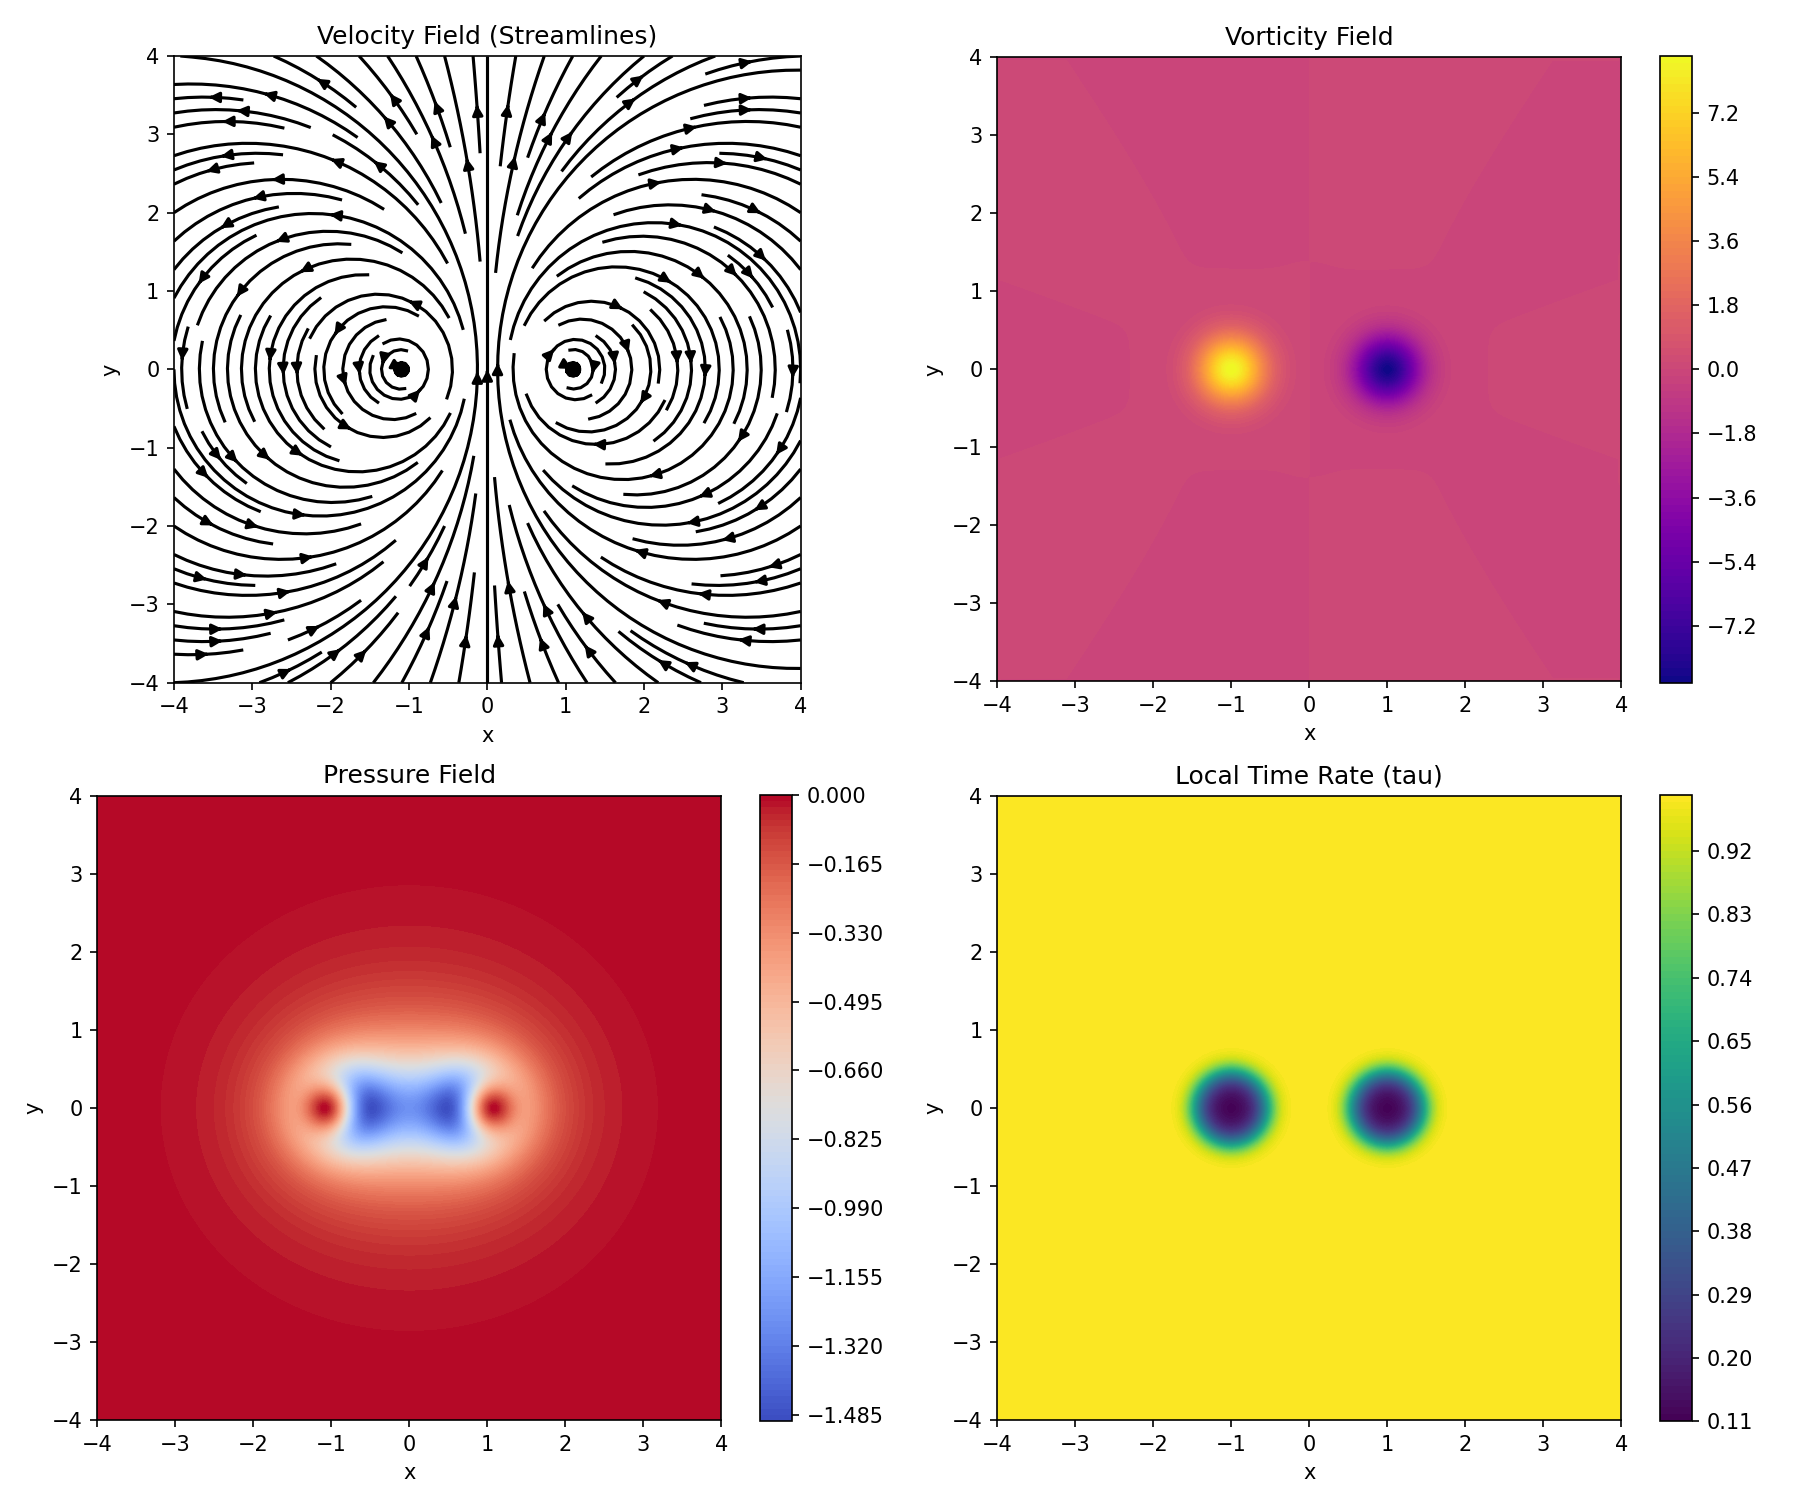
\includegraphics[width=0.85\textwidth]{streamlinesDiPole}
    \caption{Velocity streamlines, vorticity, pressure, and local time rate $\tau$ for a simulated vortex pair. The pressure minimum and time slow-down clearly align with the regions of high vorticity. This directly illustrates the æther model's central claim: time dilation follows from vortex energetics and pressure depletion.}
    \label{fig:vortexfields}
\end{figure}

\subsection{Bernoulli Flow and Local Time Depletion}

In a classical, inviscid, incompressible fluid, Bernoulli's equation describes the conservation of energy in a flow:

\begin{equation}
    \frac{1}{2} \rho_{\text{\ae}}  v^2 + p = p_0 \Rightarrow p = p_0 - \frac{1}{2} \rho_{\text{\ae}} v^2\label{eq:bernoulli}
\end{equation}

Here:
\begin{itemize}
    \item $p_0$ is the background reference pressure,
    \item $\rho_{\text{\ae}}$ is the constant æther density,
    \item $v$ is the local velocity of the æther near the vortex.
\end{itemize}

Assuming that clock rate is proportional to pressure (i.e., time slows in low-pressure regions), we relate the local clock frequency to the background as:

\begin{equation}
    \frac{f_{\text{local}}}{f_0} = 1 - \frac{\rho_{\text{\ae}} v^2}{2 p_0}\label{eq:local_clock_frequency}
\end{equation}

Hence, time dilation is:

\begin{equation}
    \frac{t_{\text{local}}}{t_0} = \left(1 - \frac{\rho_{\text{\ae}} v^2}{2 p_0}\right)^{-1}\label{eq:time_dilation}
\end{equation}

For rotational flow, with $v = \Omega r$,

\begin{equation}
    \frac{t_{\text{local}}}{t_0} = \left(1 - \frac{\rho_{\text{\ae}} \Omega^2 r^2}{2 p_0} \right)^{-1} \approx 1 + \frac{\rho_{\text{\ae}}\Omega^2 r^2}{2 p_0}\label{eq:time_dilation_rotational}
\end{equation}

This expression recovers the first-order time dilation analog if we define the dimensionless coupling:

\begin{equation}
    \frac{\rho_{\text{\ae}}}{p_0} \sim \frac{1}{c^2}\label{eq:dimensionless_coupling}
\end{equation}

This motivates the analogy to relativistic time dilation:

\begin{equation}
    \frac{t_{\text{moving}}}{t_\text{rest}} \approx 1 + \frac{v^2}{2 c^2}\label{eq:relativistic_time_dilation}
\end{equation}

\begin{figure}[htbp]
    \centering
    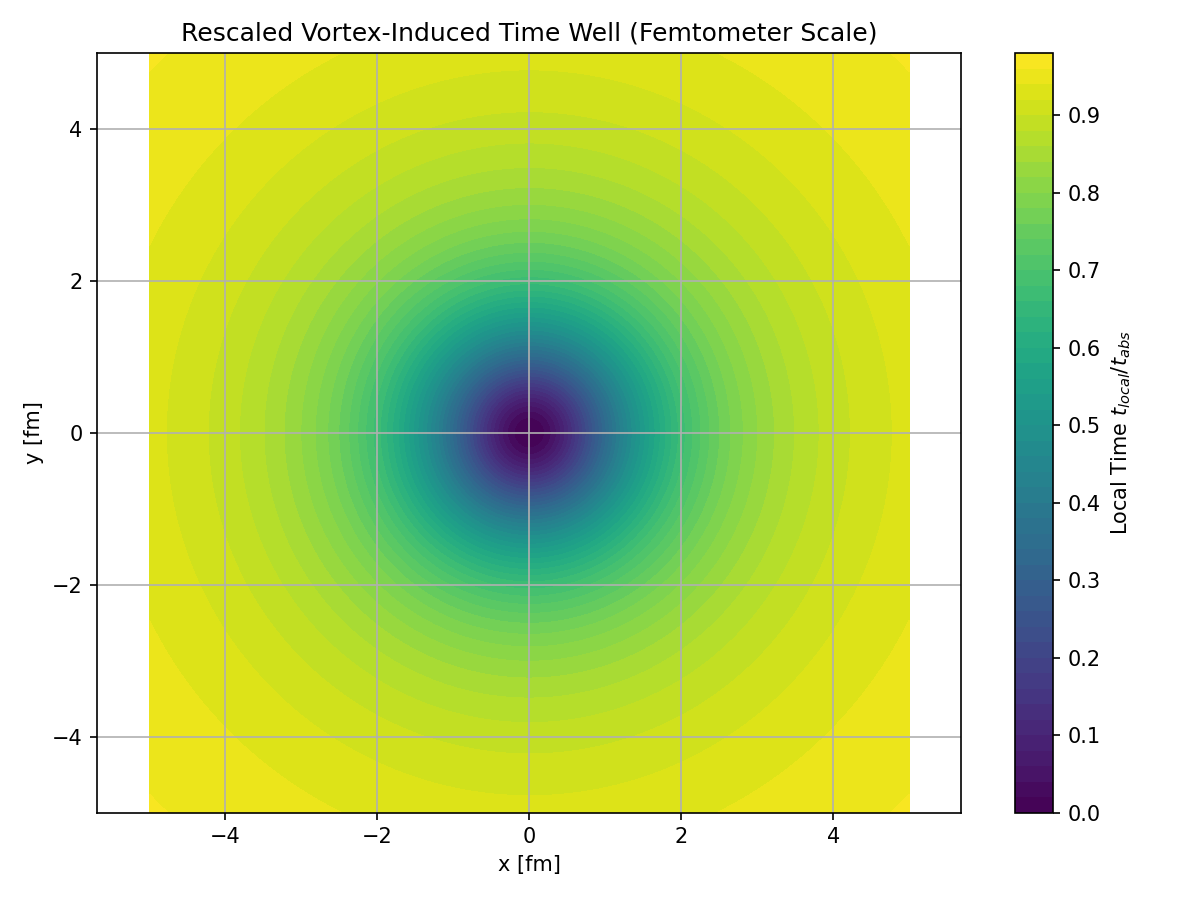
\includegraphics[width=0.8\textwidth]{RadialProfileOfLocalTimeDilation_Vortex-Induced_Time_Well}
    \caption{Schematic of a vortex-induced time well in the æther. Local time $t_{\text{local}} / t_{\text{abs}}$ is shown as a color gradient in 2D space. The central vortex region exhibits the most time slowing due to high $\Omega_k$, forming a well-like structure.}
    \label{fig:vortex_time_well}
\end{figure}


\subsection{Heuristic Knot-Based Time Modulation}

Topological vortex knots have intrinsic angular frequency $\Omega_k$, conserved due to vorticity confinement. We introduce a first-principles motivated
time dilation expression:

\begin{equation}
\frac{t_{\text{local}}}{t_{\text{abs}}} = \left(1 + \alpha \Omega_k^2 \right)^{-1}\label{eq:angular_time_dilation}
\end{equation}

where $\alpha$ is a coupling parameter with dimensions $[\alpha] = \text{s}^2$. Expanding for small $\Omega_k$:

\begin{equation}
\frac{t_{\text{local}}}{t_{\text{abs}}} \approx 1 - \alpha \Omega_k^2 + \mathcal{O}(\Omega_k^4)\label{eq:angular_time_dilation_expansion}
\end{equation}

This form parallels the Lorentz factor expansion:

\begin{equation}
\frac{t_{\text{moving}}}{t_{\text{rest}}} \approx 1 - \frac{v^2}{2 c^2}\label{eq:lorentz_time_dilation}
\end{equation}

\begin{figure}[htbp]
    \centering
    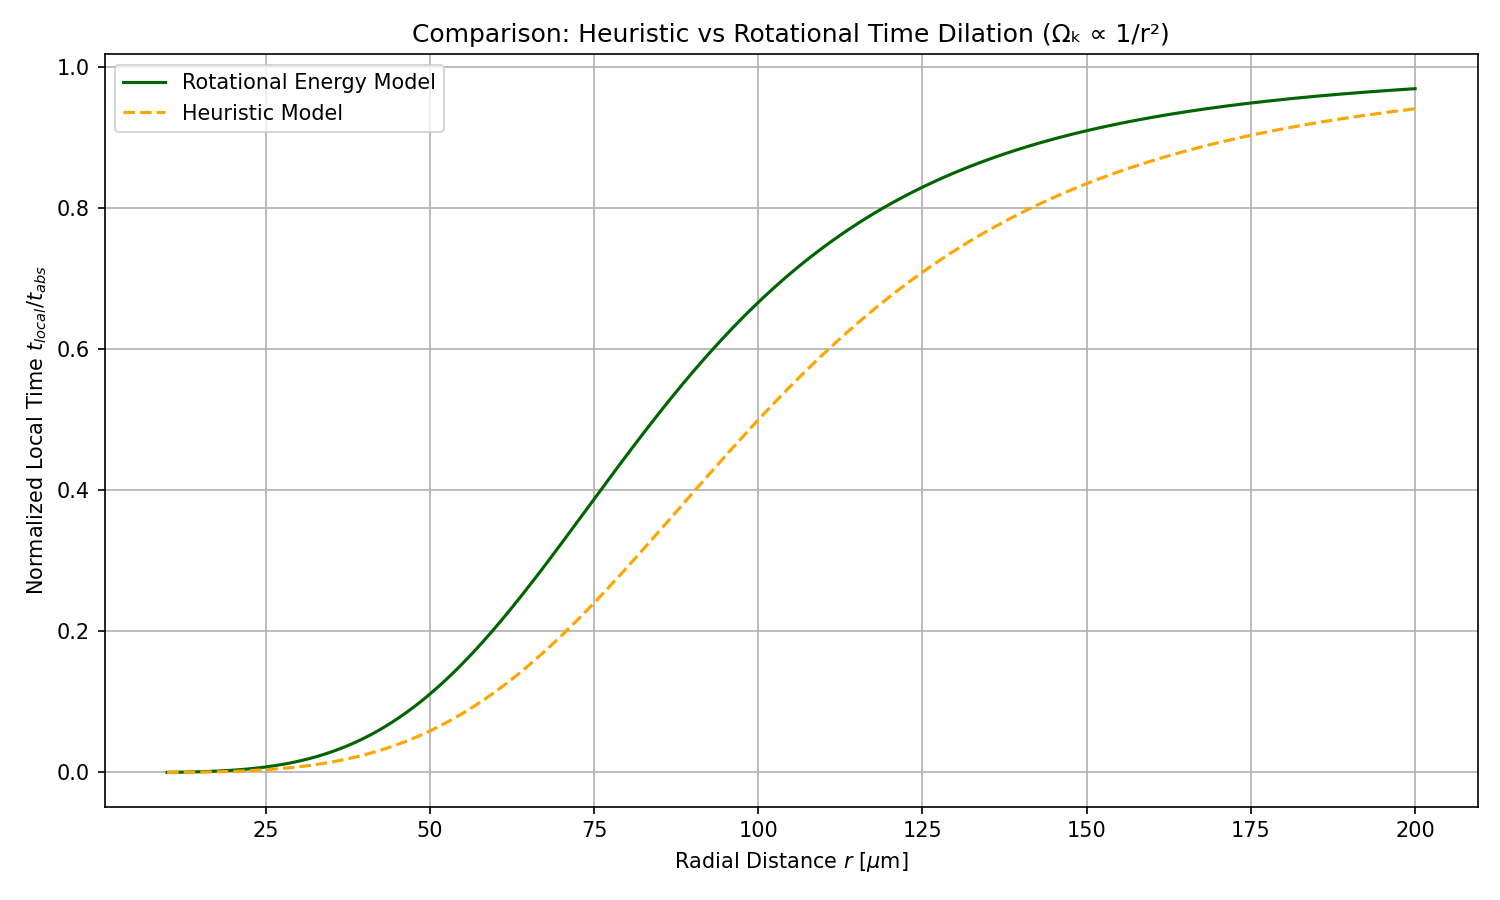
\includegraphics[width=0.8\textwidth]{RotationalVsHeuristicTimeDilation}
    \caption{\textbf{Comparison: Heuristic vs Rotational Time Dilation (\(\Omega_k \propto 1/r^2\))}.
    This graph compares two models of time modulation within the Vortex Æther framework.
    The heuristic model (green) assumes time rate reduction proportional to \((1 + \alpha \Omega_k^2)^{-1}\),
        while the rotational model (dark blue) incorporates rotational energy \(E_{\text{rot}} = \frac{1}{2} I \Omega_k^2\) and suppresses local time via
        \((1 + \frac{1}{2} \alpha I \Omega_k^2)^{-1}\). Both curves exhibit strong time dilation near the vortex core (\(r \sim 10^{-15}\) m),
        approaching absolute time flow only at extended distances. The rotational model yields a steeper suppression,
        highlighting the energetic cost of maintaining high angular momentum in fluid-based time curvature.
    }
    \label{fig:radial_time_profile}
\end{figure}

\subsection{Time Dilation from Rotational Inertia}

We now ground the heuristic form in physical energetics. For a knot with moment of inertia $I$, the rotational energy is:

\begin{equation}
E_{\text{rot}} = \frac{1}{2} I \Omega_k^2\label{eq:rotational_energy}
\end{equation}

Thus, the time dilation becomes:

\begin{equation}
\frac{t_{\text{local}}}{t_{\text{abs}}} = \left(1 + \alpha E_{\text{rot}} \right)^{-1} = \left(1 + \frac{1}{2} \alpha I \Omega_k^2 \right)^{-1}\label{eq:time_dilation_rotational_energy}
\end{equation}

This is the key result:

\begin{equation}
    \boxed{\frac{t_{\text{local}}}{t_{\text{abs}}} = \left(1 + \frac{1}{2} \alpha I \Omega_k^2 \right)^{-1}}
    \label{eq:localtime_vortex}
\end{equation}

\subsection{Summary of Model Hierarchy}

\begin{itemize}
\item Pressure-Based (Bernoulli): Time slows in low-pressure zones due to vortex velocity.
\item Heuristic Angular Model: Time slows proportionally to $\Omega_k^2$.
\item Energetic Model: Time flow depends on stored rotational energy in the knot.
\end{itemize}

These form a continuum of physical justification, culminating in a replacement of spacetime curvature with rotational æther mechanics. This establishes the VAM time dilation framework as a fluidic, topologically-conserved analog to GR.

Next, we will explore how these models correspond to GR-like metrics and rotational observers in Section II.
\section{Time modulation by rotation of vortex nodes}

Building on the discussion of time dilation via pressure and Bernoulli dynamics in the previous section, we now focus on the intrinsic rotation of topological vortex nodes. In the Vortex Æther Model (VAM), particles are modeled as stable, topologically conserved vortex nodes embedded in an incompressible, inviscid superfluid medium. Each node possesses a characteristic internal angular frequency $\Omega_k$, and this internal motion induces local time modulation with respect to the absolute time of the æther.

Instead of warping spacetime, we propose that internal rotational energy and helicity conservation cause temporal delays analogous to gravitational redshift. In this section, these ideas are developed using heuristic and energetic arguments consistent with the hierarchy introduced in Section I.

\subsection{Heuristic and energetic derivation}

We start by proposing a rotational induced time dilation formula based on the internal angular frequency of the node:

\begin{equation}
    \frac{t_\text{local}}{t_\text{abs}} = \left(1 + \beta \Omega_k^2 \right)^{-1}\label{eq:rotational_induced_time_dilation}
\end{equation}

where:

\begin{itemize}
    \item $t_\text{local}$ is the proper time near the node,
    \item $t_\text{abs}$ is the absolute time of the background æther,
    \item $\Omega_k$ is the mean core angular frequency,
    \item $\beta$ is a coupling coefficient with dimensions $[\beta] = \text{s}^2$.
\end{itemize}

For small angular velocities we obtain a first-order expansion:

\begin{equation}
    \frac{t_\text{local}}{t_\text{abs}} \approx 1 - \beta \Omega_k^2 + \mathcal{O}(\Omega_k^4)\label{eq:rotational_induced_time_dilation_expansion}
\end{equation}

This form parallels the Lorentz factor at low velocities in special relativity:

\begin{equation}
    \frac{t_\text{moving}}{t_\text{rest}} \approx 1 - \frac{v^2}{2c^2}\label{eq:parallels_lorentz_time_dilation}
\end{equation}

This yields a important analogy: Internal rotational motion in VAM induces time dilation, similar to how translational velocity induces time dilation in SR.

To strengthen the physical basis of this expression, we now relate time dilation to the energy stored in vortex rotation. Suppose the vortex node has an effective moment of inertia $I$. The rotational energy is given by:

\begin{equation}
    E_\text{rot} = \frac{1}{2} I \Omega_k^2\label{eq:rotational_energy_inertia}
\end{equation}

Assuming that time slows down due to this energy density, we write:

\begin{equation}
    \frac{t_\text{local}}{t_\text{abs}} = \left(1 + \beta E_\text{rot} \right)^{-1} = \left(1 + \frac{1}{2} \beta I \Omega_k^2 \right)^{-1}\label{eq:time_dilation_rotational_energy_inertia}
\end{equation}

This expression serves as the energetic analogue of the pressure-based Bernoulli model from Section I (cf. ~\eqref{eq:vortex_time_dilation}). It supports the interpretation of vortex-induced time wells via energy storage rather than geometric deformation.

\subsection{Topological and physical justification}

Topological vortex nodes are characterized not only by rotation, but also by helicity:

\begin{equation}
    H = \int \vec{v} \cdot \vec{\omega} \, d^3x \label{eq:helicity_rotation}
\end{equation}

Helicity is a conserved quantity in ideal (invisible, incompressible) fluids, which encodes the connection and rotation of vortex lines. The rotation frequency $\Omega_k$ becomes a topologically meaningful indicator of the identity and dynamic state of the node.

Higher $\Omega_k$ values indicate more rotational energy and deeper pressure wells, leading to transient delays that resemble gravitational redshift, but without spacetime curvature.

Each particle is a topological vortex knot:
\begin{itemize}
    \item Charge $\leftrightarrow$ rotation or chirality of the knot
    \item Mass $\leftrightarrow$ integrated vorticity energy
    \item Spin $\leftrightarrow$ knot helix:
\end{itemize}
Stability $\leftrightarrow$ knot type (Hopf connections, Trefoil, etc.) and energy minimization in the vortex core

This model:

\begin{itemize}
    \item Attributes time modulation to conserved, intrinsic rotational energy,
    \item Requires no external frames of reference (absolute æther time is universal),
    \item Preserves temporal isotropy outside the vortex core,
    \item Provides a natural replacement for the spacetime curvature of GR. \end{itemize}

Therefore, this vortex-energetic time dilation principle provides a powerful alternative to relativistic time modulation by anchoring all temporal effects in rotational energetics and topological invariants.

In the next section, we will show how these ideas reproduce metric-like behavior for rotating observers, including a direct fluid-mechanical analogue to the Kerr metric of general relativity.
\input{03_Proper_Time_for_a_Rotating_Observer_in_Æther_Flow}
\section{Kerr-like time adjustment based on vorticity and circulation}

To complete the analogy between general relativity (GR) and the vortex-æther model (VAM), we now derive a time modulation formula that reflects the redshift and frame-dragging structure in the Kerr solution. In GR, the Kerr metric describes the spacetime geometry around a rotating mass and predicts both gravitational time dilation and frame-dragging due to angular momentum. VAM captures similar phenomena via the dynamics of structured vorticity and circulation in the æther, without the need for spacetime curvature.

\subsection{General relativistic Kerr redshift structure}

In the GR-Kerr metric, the proper time $d\tau$ for an observer near a rotating mass is affected by both mass-energy and angular momentum. A simplified approximation for the time dilation factor near a rotating body is:
\begin{equation}
    t_{\text{adjusted}} = \Delta t \cdot \sqrt{1 - \frac{2GM}{rc^2} - \frac{J^2}{r^3c^2}}
    \label{eq:Kerr_time_dilation}
\end{equation}
where:
\begin{itemize}
    \item $M$: mass of the rotating body,
    \item $J$: angular momentum,
    \item $r$: radial distance from the source,
    \item $G$: Newton's gravitational constant,
    \item $c$: speed of light.
\end{itemize}

The first term corresponds to gravitational redshift with respect to the mass, while the second takes into account rotational effects (frame-dragging).

\subsection{Æther analogous via vorticity and circulation}

In VAM we express gravitational influences via vorticity intensity $\langle \omega^2 \rangle$ and total circulation $\kappa$. These are interpreted as:
\begin{itemize}
    \item $\langle \omega^2 \rangle$: mean square vorticity over a region,
    \item $\kappa$: conserved circulation, encoding angular momentum.

\end{itemize}

We define the æther-based analogue by performing the following replacements:
\begin{equation}
    \begin{aligned}
        \frac{2GM}{rc^2} &\rightarrow \frac{\gamma \langle \omega^2 \rangle}{rc^2}, \\
        \frac{J^2}{r^3c^2} &\rightarrow \frac{\kappa^2}{r^3c^2}
    \end{aligned}
    \label{eq:Kerr_replacements}
\end{equation}

Here $\gamma$ is a coupling constant relating the vorticity to the effective gravity (analogous to $G$). The æther-based proper then becomes:

\begin{equation}
    \boxed{t_{\text{adjusted}} = \Delta t \cdot \sqrt{1 - \frac{\gamma \langle \omega^2 \rangle}{rc^2} - \frac{\kappa^2}{r^3c^2}}}
    \label{eq:Kerr_time_dilation_ae}
\end{equation}

This reflects the Kerr redshift and frame dragging structure using fluid dynamic variables. In this figure:
\begin{itemize}
    \item $\langle \omega^2 \rangle$ plays the role of energy density that produces gravitational redshift,
    \item $\kappa$ represents angular momentum that generates temporal frame-dragging,
    \item The equation reduces to a flat æther time ($t_{\text{adjusted}} \tot \Delta t$) when both terms vanish.

\end{itemize}

\subsection*{Hybrid VAM Frame-Dragging Angular Velocity}

In the Vortex Æther Model (VAM), the frame-dragging angular velocity induced by a rotating vortex-bound object is defined analogously to the Lense-Thirring effect in general relativity, but with a scale-dependent Coupling:

\begin{equation}
    \omega_{\text{drag}}^{\text{VAM}}(r) =
    \frac{4 G m}{5 c^2 r} \cdot \mu(r) \cdot \Omega(r)
\end{equation}

Where \( G \) is the gravitational constant, \( c \) is the speed of light, \( m \) is the mass of the object, \( r \) is the characteristic radius, and \( \Omega(r) \) the angular velocity.

The hybrid coupling factor \( \mu(r) \) interpolates between quantum-scale vortex behavior and classical macroscopic rotation:

\begin{equation}
    \mu(r) =
    \begin{cases}
        \displaystyle \frac{r_c C_e}{r^2}, & \text{if } r < r_\ast \quad \text{(quantum or vortex core regime)} \\
        1, & \text{if } r \geq r_\ast \quad \text{(macroscopic regime)}
    \end{cases}
\end{equation}

where:
\begin{itemize}
    \item \( r_c \) is the radius of the vortex core,
    \item \( C_e \) is the tangential velocity of the vortex core,
    \item \( r_\ast \sim 10^{-3} \, \text{m} \) is the transition radius between microscopic and macroscopic regimes.
\end{itemize}

This formulation provides continuity with GR predictions for celestial bodies, while allowing VAM-specific predictions for elementary particles and subatomic vortex structures.

\subsection*{VAM Gravitational Redshift from Core Rotation}

In the Vortex Æther Model (VAM), gravitational redshift arises from the local rotation velocity \( v_\phi \) at the outer boundary of a vortex node. Assuming no spacetime curvature and absolute time, the effective gravitational redshift is given by:

\begin{equation}
    z_{\text{VAM}} =
    \left( 1 - \frac{v_\phi^2}{c^2} \right)^{-\frac{1}{2}} - 1
\end{equation}

where:
\begin{itemize}
    \item \( v_\phi = \Omega(r) \cdot r \) is the tangential velocity due to local rotation,
    \item \( \Omega(r) \) is the angular velocity at the measurement beam \( r \),
    \item \( c \) is the speed of light in vacuum.

\end{itemize}

This expression reflects the change in time perception caused by local rotational energy, replacing the curvature-based gravitational potential \( \Phi \) of general relativity with a velocity field term. It becomes equivalent to the GR Schwarzschild redshift for low \( v_\phi \) and diverges as \( v_\phi \rightarrow c \), which provides a natural limit to the evolution of the local frame:

\begin{equation}
    \lim_{v_\phi \to c} z_{\text{VAM}} \to \infty
\end{equation}

\subsection*{VAM Local Time Dilation Models}

In the Vortex Æther Model (VAM), local time dilation is interpreted as the modulation of absolute time by internal vortex dynamics, not by spacetime curvature. Depending on the system scale, two physically based formulations are used:

\paragraph{1. Time dilation based on velocity fields}

This model relates the local time flow to the tangential speed of the rotating etheric structure (vortex node, planet or star):

\begin{equation}
    \frac{d\tau}{dt} =
    \sqrt{1 - \frac{v_\phi^2}{c^2}} =
    \sqrt{1 - \frac{\Omega^2 r^2}{c^2}}
\end{equation}

whereby:
\begin{itemize}
    \item \( v_\phi = \Omega \cdot r \) is the tangential speed,
    \item \( \Omega \) is the angular velocity at radius \( r \),
    \item \( c \) is the speed of light.
\end{itemize}

\paragraph{2. Time dilation based on rotational energy}

On large scales or with high rotational inertia, time dilation arises from stored rotational energy, leading to:

\begin{equation}
    \frac{d\tau}{dt} =
    \left(1 + \frac{1}{2} \cdot \beta \cdot I \cdot \Omega^2 \right)^{-1}
\end{equation}

with:
\begin{itemize}
    \item \( I = \frac{2}{5} m r^2 \): moment of inertia for a uniform sphere,
    \item \( \beta = \frac{r_c^2}{C_e^2} \): coupling constant of vortex-core dynamics,
    \item \( m \) is the mass of the object. \end{itemize}

\paragraph{Interpretation}

These models imply that time slows down in regions of high local rotational energy or vorticity, consistent with gravitational time dilation effects in GR. In VAM, however, these effects arise exclusively from the internal dynamics of the æther flow, under flat 3D Euclidean geometry and absolute time.

\subsection{Model assumptions and scope}

This result depends on several assumptions:
\begin{itemize}
    \item The flow is irrotational outside the vortex cores,
    \item Viscosity and turbulence are neglected,
    \item Compressibility is ignored (ideal incompressible superfluid),
    \item Vorticity fields are sufficiently smooth to define $\langle \omega^2 \rangle$.
\end{itemize}

These conditions reflect the assumptions of analogous models of ideal fluid GR. The formulation bridges the macroscopic fluid dynamics of the æther with effective geometric predictions, which strengthens the possibility of replacing curved spacetime with structured vorticity fields.

See Appendix~\ref{appendix:7} for detailed derivations of cross-energy and vortex interaction energetics.

In future work, corrections for boundary conditions, quantized vorticity spectra, and compressibility effects can be added to refine the analogy. We then summarize how these fluid-based time dilation mechanisms coalesce within the VAM framework and identify their experimental implications.
\section{Unified Framework and Synthesis of Time Dilation in VAM}

This section unifies the time dilation mechanisms discussed in the paper under the Vortex Æther Model (VAM). Instead of relying on spacetime curvature, VAM attributes temporal effects to classical fluid dynamics, rotational energy, and topological vorticity.

\subsection{Hierarchical Structure of Time Dilation Mechanisms}

Each section of this work contributes a separate but interrelated mechanism for time dilation:

\begin{enumerate}
    \item \textbf{Bernoulli-Induced Time Depletion:} Time slows down near regions of low pressure due to vortex-induced kinetic velocity fields. This results in a special relativistic time dilation form when \( \rho_{\text{\ae}} / p_0 \sim 1/c^2 \).
    \item \textbf{Heuristic model for angular frequency:} A quadratic dependence of the time velocity on the local nodal angular frequency \( \Omega_k^2 \), which mimics the Lorentz factor expansion for small velocities.
    \item \textbf{Energetic formulation via rotational inertia:}
    \[
        \boxed{\frac{t_{\text{local}}}{t_{\text{abs}}} = \left(1 + \frac{1}{2} \beta I \Omega_k^2 \right)^{-1}}
    \]
    directly links time modulation to the rotational energy of vortex nodes. \item \textbf{Own time stream based on velocity field:}
    \[
        \boxed{\left( \frac{d\tau}{dt} \right)^2 = 1 - \frac{1}{c^2}(v_r + r\Omega_k)^2}
    \]
    \item \textbf{Kerr-like redshift and frame drag:}
    \[
        \boxed{t_{\text{adjusted}} = \Delta t \cdot \sqrt{1 - \frac{\gamma \langle \omega^2 \rangle}{rc^2} - \frac{\kappa^2}{r^3c^2}}}
    \]
\end{enumerate}

These five expressions form a self-consistent ladder, ranging from heuristic to rigorous, and provide a robust replacement for general relativistic time dilation, based entirely on classical field variables.

\subsection{Physical unification: Time as a vorticity-derived observable}

A recurring theme emerges in all formulations: \textit{time modulation in VAM is always reducible to local kinetic or rotational energy density within the æther}. Whether encoded in pressure (Bernoulli), angular frequency (\( \Omega_k \)) or field circulation (\( \kappa \)), the modulation of time is not geometric but energetic and topological.

\begin{itemize}
    \item Local time wells arise from high vorticity and circulation.
    \item Frame independence: Absolute time exists; only local velocities are affected.
    \item No need for tensor geometry: All time effects arise from scalar or vector fields.
    Topological conservation: Vortices preserve helicity and circulation, which provides temporal consistency.

    This unification strengthens the conceptual core of VAM: spacetime curvature is an emergent illusion caused by structured vorticity in an absolute, superfluid æther.

    Experimental implications and prospects

    Each time dilation formula introduced here can in principle be tested in analogous laboratory systems:

    Rotating superfluid droplets (e.g., helium-II, BECs)
    Electrohydrodynamic lifters and plasma vortex systems
    Magnetofluidic and optical analogs

    Future work includes:
    Establishment of items
    Deriving dynamical equations for temporal feedback in multi-node systems. \item Measuring vortex-induced clock drift in rotating superfluids.

    \item Applying the model to astrophysical observations (e.g., neutron star precession, frame dragging, time dilation).
\end{itemize}

\subsection{Challenges, limitations, and paths to broader relevance}

\textbf{Fundamental assumptions:} Reintroducing an æther with absolute time poses a challenge to a century of relativistic physics.

\textbf{Experimental validation:} There is no direct empirical evidence yet to support the proposed æther or specific dilation mechanisms.

\textbf{Reception in mainstream physics:} While niche communities may engage, mainstream physics may resist because of deviations from established frameworks.

\subsection{Enhancing scientific rigor and broader appeal}

\begin{itemize}
    \item \textbf{Propose testable predictions:} especially where VAM deviates from GR.
    \item \textbf{Integrate with established theories:} show borderline cases that match GR/QM. \item \textbf{Address historical objections:} clearly redefine æther with modern restrictions.
    \item \textbf{Peer Review and Collaboration:} invite criticism from specialists.
    \item \textbf{Clarity and Accessibility:} simplify the conceptual presentation without sacrificing precision.
\end{itemize}

\subsection{Concluding Perspective}

The Vortex Æther Model (VAM) offers a bold reinterpretation of gravitational time dilation due to vorticity-driven energetics in an absolute, superfluid medium. Through a hierarchy of derivations—encompassing Bernoulli flows, vortex rotation, energy density, and circulation—it provides a coherent alternative to relativistic, curvature-based descriptions. Although VAM departs from conventional theories, its internal logic and conceptual clarity warrant further investigation. Continued refinement, integration, and empirical testing will determine what role the technology will play in further deepening our understanding of gravity, time, and the structure of the universe.
%! Author = mr
%! Date = 3/29/2025


\section{VAM Vortex Scattering Framework (Inspired by Elastic Theory)}

\subsection{Governing Equations of VAM Vorticity Dynamics}

\subsubsection*{Vorticity Transport Equation (Linearized Form)}

In the Vortex Æther Model (VAM), the dynamics of the vorticity field \(\vec{\omega} = \nabla \times \vec{v}\) are governed by the Euler equation and its vorticity form:

\[
\frac{\partial \omega_i}{\partial t} + v_j \partial_j \omega_i = \omega_j \partial_j v_i
\]

This nonlinear structure implies vortex deformation due to stretching and advection. For small perturbations \(\delta\omega\) near a background vortex knot field \(\omega^{(0)}\), linearization gives:

\[
\frac{\partial (\delta \omega_i)}{\partial t} + v_j^{(0)} \partial_j (\delta \omega_i) \approx \omega_j^{(0)} \partial_j (\delta v_i)
\]

Define the VAM linear response operator \(\mathcal{L}_{ij}\):

\[
\mathcal{L}_{ij} \, \delta v_j(\vec{r}) = \delta F_i^{\text{vortex}}(\vec{r})
\]

\subsubsection*{Vorticity Green Tensor Equation}

\[
\mathcal{L}_{ij} \, \mathcal{G}_{jk}(\vec{r}, \vec{r}') = -\delta_{ik} \, \delta(\vec{r} - \vec{r}')
\]

The induced velocity field \(v_i\) from a source vortex forcing \(F_k(\vec{r}')\) is then:

\[
v_i(\vec{r}) = \int \mathcal{G}_{ik}(\vec{r}, \vec{r}') \, F_k^{\text{vortex}}(\vec{r}') \, d^3 r'
\]

\subsection{Vortex Thread Interaction}
Interactions arise from exchange of vorticity or reconnections between vortex filaments:
\begin{itemize}
    \item Attractive if threads reinforce circulation (parallel)
    \item Repulsive if threads cancel (antiparallel)
    \item Interaction strength:
\end{itemize}
\begin{equation}
    \vec{F}_{\text{int}} = \beta \cdot \kappa_1 \kappa_2 \cdot \frac{\vec{r}_{12} \times (\vec{v}_1 - \vec{v}_2)}{|\vec{r}_{12}|^3}\label{eq:interaction_strength}
\end{equation}
Where \(\kappa_i\) are circulations of filaments and \(\vec{r}_{12}\) is the vector between them.

\subsection{Thermodynamic \& Quantum Behavior from Vorticity Fluctuations}
\begin{itemize}
    \item Entropy \(\leftrightarrow\) volume of vortex expansion or knot deformation
    \item Quantum transitions \(\leftrightarrow\) topological reconnection events
    \item Zero-point motion \(\leftrightarrow\) background quantum turbulence of the Æther:
\end{itemize}

\subsubsection*{Quantum Vorticity Background}
\begin{equation}
    \langle \omega^2 \rangle \sim \frac{\hbar}{\rho_\text{æ} \xi^4}\label{eq:quantum_vorticity_background}
\end{equation}
Where \(\xi\) is the coherence length between vortex filaments.

\subsection{VAM Scattering Theory for Vortex Knots}

\subsubsection*{Born Approximation for Vorticity Perturbations}

Assume an incident vorticity potential \(\Phi^{(0)}(\vec{r})\) encounters a vortex knot at \(\vec{r}_k\). The scattered vorticity field becomes:

\[
\Phi(\vec{r}) = \Phi^{(0)}(\vec{r}) + \int \mathcal{G}_{ij}(\vec{r}, \vec{r}') \, \delta \mathcal{V}_{jk}(\vec{r}') \, v_k^{(0)}(\vec{r}') \, d^3r'
\]

Here, \(\delta \mathcal{V}_{jk}\) represents a vorticity polarizability tensor associated with the knot—a VAM analog to elastic moduli perturbation.

\subsection{Æther Stress Tensor and Energy Flux}

\subsubsection*{VAM Stress Tensor}

\[
\mathcal{T}_{ij} = \rho_{\text{\ae}} \, v_i v_j - \frac{1}{2} \delta_{ij} \rho_{\text{\ae}} v^2
\]

\subsubsection*{Æther Vorticity Force Density}

\[
f_i^{\text{vortex}} = \partial_j \mathcal{T}_{ij}
\]

\subsubsection*{Vorticity Energy Flux}

\[
\vec{S}_\omega = - \mathcal{T} \cdot \vec{v}
\]

This vector captures energy transfer through vortex knot interactions and defines scattering "cross sections" via the divergence \(\nabla \cdot \vec{S}_\omega\).

\subsection{Time Dilation and Knot Scattering}

\subsubsection*{Time Dilation from Knot Rotation}

Let the incident vorticity field induce localized time slowing due to a knot’s rotational energy:

\[
\frac{t_{\text{local}}}{t_{\infty}} = \left(1 + \frac{1}{2} \beta I \Omega_k^2 \right)^{-1}
\]

In the Born approximation, the change in proper time near a knot under external vorticity flow is:

\subsubsection*{Scattered Correction from External Field}

\begin{gather*}
    \delta \left( \frac{t_{\text{local}}}{t_{\infty}} \right) \approx - \frac{1}{2} \beta I \Omega_k \, \delta \Omega_k\\
    \delta \Omega_k \sim \int \chi(\vec{r}_k - \vec{r}') \cdot \vec{\omega}^{(0)}(\vec{r}') \, d^3r'\\
\end{gather*}

Here, \(\chi\) is the topological vortex susceptibility kernel.



\subsection{Summary of VAM-Inspired Scattering Constructs}


\begin{table}[htbp]
    \centering
    \begin{tabular}{lll}
        \toprule
        \textbf{Concept} & \textbf{Elastic Theory} & \textbf{VAM Analog} \\
        \midrule
        Medium property & \( c_{ijkl} \) & \( \rho_{\text{\ae}},\, \Omega_k,\, \kappa \) \\
        Wavefield & \( u_i \) (displacement) & \( v_i \) (Æther velocity) \\
        Source & \( f_i \) (body force) & \( F_i^{\text{vortex}} \) (vorticity forcing) \\
        Green function & \( G_{ij}(\vec{r}, \vec{r}') \) & \( \mathcal{G}_{ij}(\vec{r}, \vec{r}') \) \\
        Stress tensor & \( \tau_{ij} \) & \( \mathcal{T}_{ij} \) \\
        Energy flux & \( J_{P,i} = -\tau_{ij} \dot{u}_j \) & \( S_{\omega,i} = -\mathcal{T}_{ij} v_j \) \\
        Time dilation mechanism & \( g_{\mu\nu} \) (GR metric) & \( \Omega_k,\, \kappa,\, \langle \omega^2 \rangle \) \\
        \bottomrule
    \end{tabular}
    \caption{Conceptual correspondence between classical elasticity and Vortex Æther Model (VAM).}
    \label{tab:elastic-vam-analogy}
\end{table}



This scattering framework generalizes classical elastic analogs into a topologically and energetically motivated Ætheric formalism. It enables the computation of field modifications, time dilation effects, and energy flux due to stable, interacting vortex knots in the Vortex Æther Model (VAM).
\section{Experimental Anchors and VAM Predictions}


To assess the empirical validity of the Vortex Æther Model (VAM), we identify several high-impact experimental domains where VAM-specific signatures could be observed:

\subsection{Time Drift in Rotating Superfluid Systems.} VAM predicts localized time dilation proportional to vortex knot angular frequency
$\Omega_k$. Bose–Einstein condensates (BECs) or rotating helium droplets with embedded atomic clocks could display measurable time drift or dephasing relative to non-rotating controls.

\subsection{Plasma Vortex Clocks and Cyclotron Experiments.} Plasma devices exhibiting structured rotational flows may serve as analogs to Ætheric time wells. Phase-shift detection near plasma vortices or charged ring currents could reveal Æther-based time modulation effects.

\subsection{LENR via Resonant Vortex Knot Fusion in Pd/D Lattices.} As derived in the thermodynamic section, VAM suggests fusion-like energy release can occur when trapped vortex knots resonate with external electromagnetic fields. Measurable indicators include:
\begin{itemize}
    \item RF-tuned excess heat events
    \item Helium-4 without neutron/gamma emission
    \item Lattice transmutation signatures with no standard nuclear byproducts
\end{itemize}

\subsection{Optical and Metamaterial Simulations.} Synthetic waveguide systems or metamaterials could simulate Ætheric flow. Measuring light pulse propagation under simulated vorticity gradients may test time modulation without invoking curvature.

\subsection{Summary of VAM Observables.}
\begin{itemize}
    \item Critical thresholds for vortex collapse and energy release
    \item Temporal anomalies in rotating systems
    \item Absence of relativistic particles in high-energy fusion-like events
    \item Clock-rate asymmetries across vorticity gradients
\end{itemize}

\bibliography{citations}
\bibliographystyle{unsrtnat}

\appendix \label{sec:Part-6}
\section{ Foundations of Velocity Fields and Energies in a Vortex System.}

\subsection{abstract}
This article outlines theoretical foundations of vortical velocity fields and their associated energies,
including a distinction between self- and cross-energies, in the context of a generic vortex-based model.
We close with a derivation outline for the cross-energy term, highlighting its application in vortex dynamics
and fluid–structure interactions.

\subsection{Introduction}
Vortex dynamics are a core component of many fluid and plasma systems, including
tornado-like flows, knotted vortices in classical or superfluid turbulence, and various
complex topological fluid systems. A deeper understanding of the energy budgets
associated with these flows can shed light on processes like vortex stability, reconnection,
and global flow organization. We begin by motivating how velocity fields can be
decomposed so as to capture the total energy (i.e.\ self- plus cross-energy), and how
this approach helps track flows in both 2D and 3D.

\subsection{Foundations: Velocity Fields and Total (Self + Cross) Energy}
\label{sec:foundations}
In an incompressible fluid, the velocity field $\mathbf{u}(\mathbf{x}, t)$ is typically
governed by the Navier--Stokes or Euler equations. For inviscid analyses, the Euler
equations for incompressible flow read
\begin{equation}
  \frac{\partial \mathbf{u}}{\partial t} + (\mathbf{u} \cdot \nabla)\mathbf{u} = -\frac{1}{\rho}\nabla p,
  \quad \nabla \cdot \mathbf{u} = 0.
\end{equation}
We also consider the vorticity $\boldsymbol{\omega} = \nabla \times \mathbf{u}$,
which can be used to characterize vortex structures.

To understand the \emph{total} kinetic energy, we can split it as follows:
\begin{equation}
  E_{\text{total}} \;=\; E_{\text{self}} \;+\; E_{\text{cross}}.
\end{equation}
Here, $E_{\text{self}}$ is that portion of energy which each vortex or partial flow
element contributes independently (for instance, from local swirling motions), while
$E_{\text{cross}}$ encodes the contributions that arise from the interaction of different
vortical elements. In a multi-vortex scenario, such a decomposition helps isolate the
direct interaction between two (or more) vortex filaments or sheets.

\subsection{Momentum and Self-Energy Considerations}
\label{sec:momentum}
A starting point is to recall that for a single vortex of circulation $\Gamma$, with an
azimuthally symmetric core, the induced velocity is sometimes approximated by
classical results such as
\begin{equation}
   V \;=\; \frac{\Gamma}{4 \pi R}
   \bigl(\ln \tfrac{8 R}{a} - \beta \bigr),
\end{equation}
where $R$ is the main vortex loop radius, $a \ll R$ is a measure of core thickness,
and $\beta$ depends on details of the core model \cite{Saffman1992}. The
\emph{self-energy} associated with that vortex, $E_{\text{self}}$, can be cast in a
similar form that depends on $\ln(R/a)$, exemplifying how thin-core vortices'
energies scale with geometry.

In more general fluid or vortex-lattice models, we can track $E_{\text{self}}$ as the
sum of individual core energies. Further, the presence of multiple filaments modifies
the total energy by cross-terms of the velocity fields (the cross-energy). This
cross-energy often drives key phenomena such as vortex merging or the `recoil'
effects in wave--vortex interactions.

\subsection{Defining and Tracking Cross-Energy}
\label{sec:cross}
When multiple vortices (or partial velocity distributions) co-exist, the total velocity
field $\mathbf{u}$ can be superposed:
\begin{equation}
   \mathbf{u} \;=\; \mathbf{u}_1 \;+\;\mathbf{u}_2,
\end{equation}
where $\mathbf{u}_1$ and $\mathbf{u}_2$ come from distinct sub-systems. In that
scenario, the kinetic energy for a fluid volume $V$ is
\begin{align}
   E_{\text{total}} &= \frac{\rho}{2} \int_V \mathbf{u}^2 \,dV
   = \frac{\rho}{2} \int_V \bigl(\mathbf{u}_1 + \mathbf{u}_2 \bigr)^2\, dV \\
   &= \frac{\rho}{2} \int_V \mathbf{u}_1^2 \,dV \;+\;\frac{\rho}{2} \int_V \mathbf{u}_2^2 \, dV
   \;+\;\rho \int_V \mathbf{u}_1 \cdot \mathbf{u}_2 \, dV,
\end{align}
revealing an interaction or \emph{cross-energy} term
\begin{equation}
   E_{\text{cross}} \;=\; \rho \int_V \mathbf{u}_1 \cdot \mathbf{u}_2 \, dV.
   \label{eq:cross-term}
\end{equation}
Much of the interesting physics arises from \eqref{eq:cross-term}, because it
grows or shrinks depending on the vortex geometry and distance between them.
Its dynamical evolution can lead to, e.g., merging or rebound. A main point is that
each vortex's self-velocity can significantly affect the mutual velocities and thus
create net forces or torque.

\subsection{Applications to Helicity and Topological Flows}
\label{sec:helicity}
A related concept is helicity, measuring the topological complexity (knotting or
linking) of vortex tubes. Classically, helicity $H$ is given by
\begin{equation}
   H \;=\; \int_V \mathbf{u} \cdot \boldsymbol{\omega}\, dV,
\end{equation}
which can remain constant or be partially lost during reconnection events. In certain
dissipative flows, the cross-energy terms in \eqref{eq:cross-term} can influence
the effective rate of helicity change. Understanding $E_{\text{cross}}$ is important
for analyzing reconnection pathways in classical or superfluid turbulence.

\subsection{Derivation Outline for Cross-Energy}
\label{sec:derivation}
Finally, we provide a succinct outline for deriving the cross-energy expression.
Starting with the total velocity field $\mathbf{u} = \sum_{n=1}^N \mathbf{u}_n$
for $N$ vortex or partial velocity fields, the total kinetic energy is:
\begin{equation}
   E_{\text{total}}
   = \frac{\rho}{2} \int_V \left(\sum_{n=1}^N \mathbf{u}_n \right)^2 dV
   = \frac{\rho}{2} \sum_{n=1}^N \int_V \mathbf{u}_n^2 \, dV
      \;+\;\rho \sum_{n<m} \int_V \mathbf{u}_n \cdot \mathbf{u}_m \, dV.
\end{equation}
One obtains $N$ self-energy terms plus pairwise cross-energy integrals.
The cross-energy for a pair $(i,j)$ is:
\begin{equation}
   E_{\text{cross}}^{(ij)} \;=\; \rho \int_V \mathbf{u}_i \cdot \mathbf{u}_j \, dV.
\end{equation}
In practice, each $\mathbf{u}_n$ may be represented by known solutions of the
Stokes or potential flow equations, or from approximate solutions for vortex loops.
Then, either analytically or numerically, one obtains approximate cross-energies
that can be used in reduced models describing the evolution of multi-vortex
systems.

\subsection*{Conclusion}
We have surveyed how the total fluid kinetic energy in the presence of multiple
vortices can be split into self- and cross-energy terms. These cross-energy
contributions are crucial for understanding vortex merging, knotted vortex
untangling, or vortex–wave interactions in classical, superfluid, and plasma
flows. In addition, we have sketched a systematic derivation of cross-energy and
highlighted key aspects in discussing momentum and helicity. Future directions
include refining these expressions for axisymmetric or knotted vortices and
integrating them into large-scale models or computational frameworks.\label{appendix:1}


\section{Integration of Clausius' Heat Theory into the Vortex \AE ther Model (VAM)}

The integration of Clausius' Mechanical Theory of Heat into the Vortex \AE ther Model (VAM) extends the framework's reach into thermodynamics,
allowing a unified interpretation of energy, entropy, and quantum behavior based on structured vorticity in an inviscid superfluid-like \ae ther
medium \cite{clausius1865mechanical, maxwell1865electromagnetic, helmholtz1858integrals}.

\subsection{Thermodynamic First Principles in VAM}

The classical first law of thermodynamics is expressed as:
\begin{equation}
\Delta U = Q - W,
\end{equation}
where $\Delta U$ is the change in internal energy, $Q$ is heat added, and $W$ is work done by the system \cite{clausius1865mechanical}. Within VAM, this becomes:
\begin{equation}
\Delta U = \Delta \left( \frac{1}{2} \rho_{\text{\ae}} \int v^2 \, dV + \int P \, dV \right),
\end{equation}
with $\rho_{\text{\ae}}$ the æther density, $v$ the local velocity, and $P$ the pressure within equilibrium vortex domains \cite{vam2025unified}.

\subsection{Entropy and Structured Vorticity}

VAM posits that entropy is a function of vorticity intensity:
\begin{equation}
S \propto \int \omega^2 \, dV,
\end{equation}
where $\omega = \nabla \times v$ \cite{kelvin1867vortex}. Thus, entropy becomes a measure of topological complexity and energy dispersion encoded in the vortex network.

\subsection{Thermal Response of Vortex Knots}

Stable vortex knots embedded in equilibrium pressure surfaces behave analogously to thermodynamic systems:
\begin{itemize}
\item \textbf{Heating ($Q > 0$)} expands the knot, lowers core pressure, and increases entropy.
\item \textbf{Cooling ($Q < 0$)} contracts the knot, concentrating energy and stabilizing vorticity.
\end{itemize}
This provides a fluid-mechanical analog to gas laws under energetic input.

\subsection{Photoelectric Analogy in VAM}

Rather than invoking quantized photons, VAM interprets the photoelectric effect through vortex dynamics. A vortex must absorb enough energy to destabilize and eject its structure:
\begin{equation}
W = \frac{1}{2} \rho_{\text{\ae}} \int v^2 \, dV + P_{\text{eq}} V_{\text{eq}},
\end{equation}
where $W$ is the disintegration work threshold. If an incident wave modulates internal vortex energy beyond this, ejection occurs \cite{vam2025unified}.

The critical force for vortex ejection is:
\begin{equation}
F_{\text{max}} = \rho_{\text{\ae}} C_e^2 \pi r_c^2,
\end{equation}
with $C_e$ the vortex's edge velocity and $r_c$ its core radius. This yields a natural frequency cutoff below which no interaction occurs, akin to the threshold frequency in quantum photoelectricity \cite{einstein1905photoelectric}.

\subsection{Conclusion and Integration}

This thermodynamic extension of VAM enriches the model by embedding classical heat and entropy principles within fluid-dynamic structures. It not only bridges vortex physics with Clausius' laws but also offers a field-based reinterpretation of light-matter interactions, unifying mechanical and electromagnetic thermodynamics without discrete particle assumptions.






\subsection*{I. Vortex Knots as Particles}
Each particle is a topological vortex knot:
\begin{itemize}
    \item Charge ↔ twist or chirality of knot
    \item Mass ↔ integrated vorticity energy
    \item Spin ↔ knot helicity:
\end{itemize}
\subsection*{Helicity as Particle Identity}
\begin{equation}
    \mathcal{H} = \int \vec{v} \cdot \vec{\omega} \, d^3x
\end{equation}
Stability ↔ knot type (Hopf links, Trefoil, etc.) and energy minimization in the vortex core

\subsection*{II. Vortex Thread Interaction}
Interactions arise from exchange of vorticity or reconnections between vortex filaments:
\begin{itemize}
    \item Attractive if threads reinforce circulation (parallel)
    \item Repulsive if threads cancel (antiparallel)
    \item Interaction strength:
\end{itemize}
\begin{equation}
    \vec{F}_{\text{int}} = \beta \cdot \kappa_1 \kappa_2 \cdot \frac{\vec{r}_{12} \times (\vec{v}_1 - \vec{v}_2)}{|\vec{r}_{12}|^3}
\end{equation}
Where \(\kappa_i\) are circulations of filaments and \(\vec{r}_{12}\) is the vector between them.


\subsection*{III. Thermodynamic & Quantum Behavior from Vorticity Fluctuations}
\begin{itemize}
    \item Entropy \(\leftrightarrow\) volume of vortex expansion or knot deformation
    \item Quantum transitions \(\leftrightarrow\) topological reconnection events
    \item Zero-point motion \(\leftrightarrow\) background quantum turbulence of the Æther:
\end{itemize}
\subsection*{Quantum Vorticity Background}
\begin{equation}
    \langle \omega^2 \rangle \sim \frac{\hbar}{\rho_\text{æ} \xi^4}
\end{equation}
Where \(\xi\) is the coherence length between vortex filaments\label{appendix:2}

\end{document}